\chapter{Implementation}

In this chapter a way to implement a system like the one described in Chapter 3 will be explained by an example based on TinyOS.    

\section{General Structure}
The system is dividable into two main components. The base station, that stores and processes the data, and the motes, that collect the data. Both parts of the system need their own hard- and software to complete their tasks.  
\subsection{General Base Station}

\begin{figure}[htbp]
	\centering
    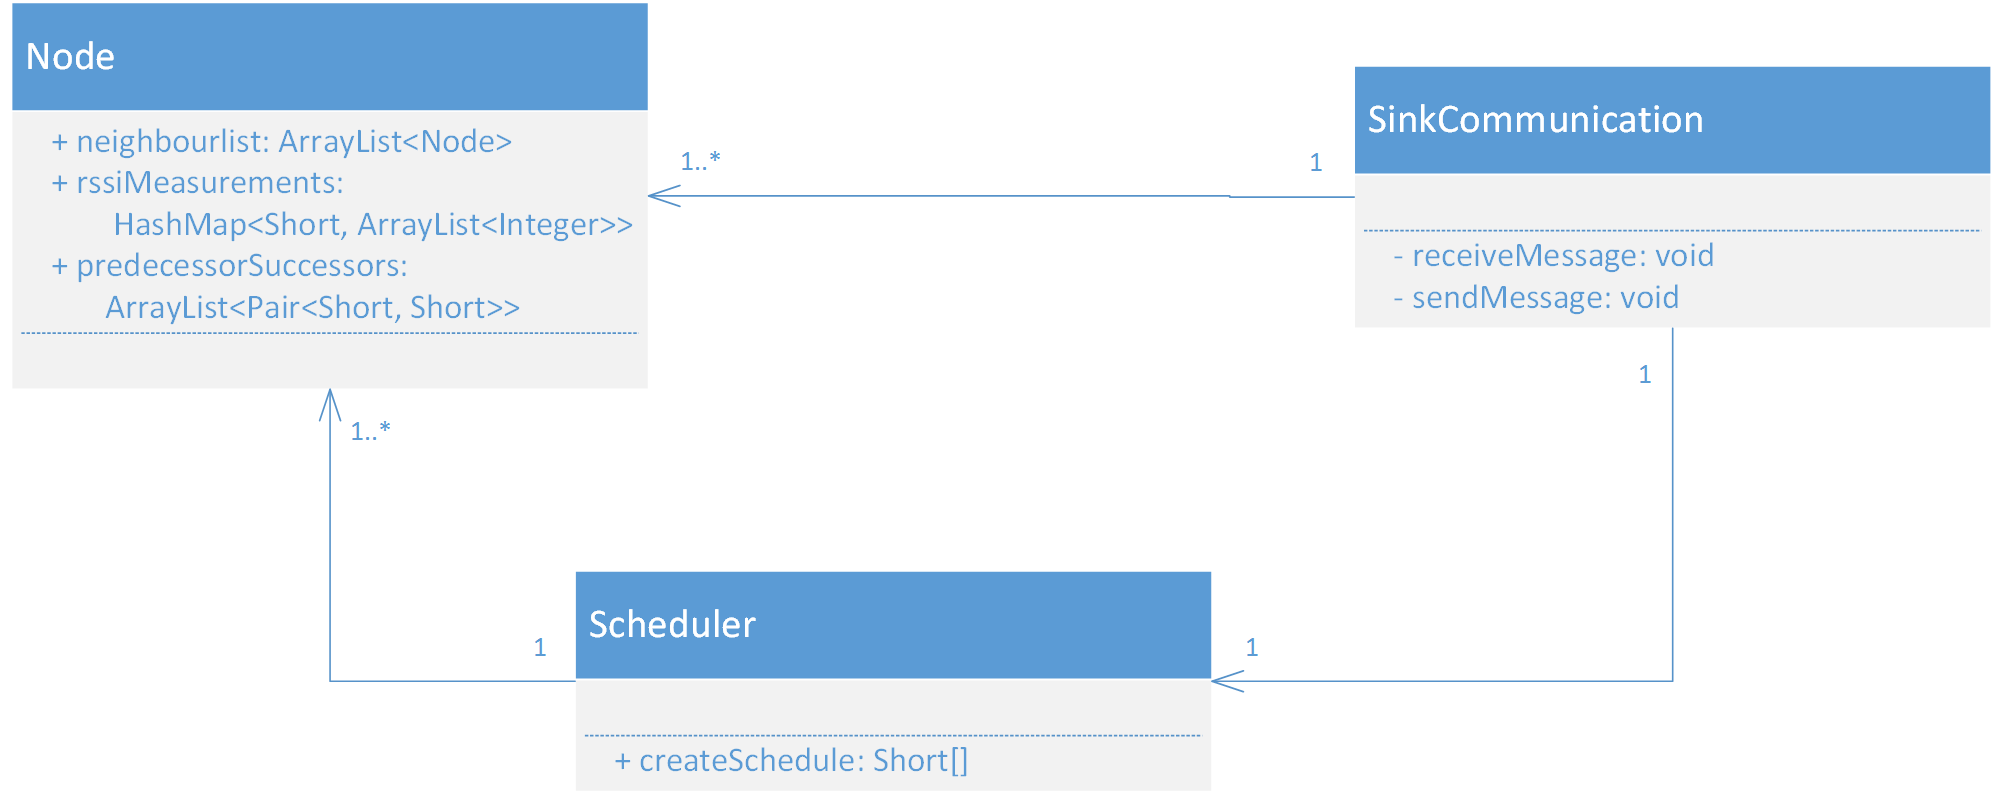
\includegraphics[scale=0.7]{content/images/BaseStation/Klassendiagram}
   	\caption{General structure and functionality of the base station}
    \label{fig:bsKlassen}
\end{figure}

The base station can be a computer running a Java application connected to the sink via a USB-Cable. In Figure \ref{fig:bsKlassen} you can see the general structure of the Java application with its classes and their basic functionality. First, there is the SinkCommunication class that handles the communication with the sink. It is responsible for receiving and processing messages and to send messages to the sink. Then there is the Node class which stores all the information about one node. It stores the neighbours of the node, the measurements a node made and its predecessors and successors. The last class is the Scheduler that is responsible of creating a schedule based on the data saved in the node classes.  
\subsection{General Mote Application}
\begin{figure}[htbp]
	\centering
    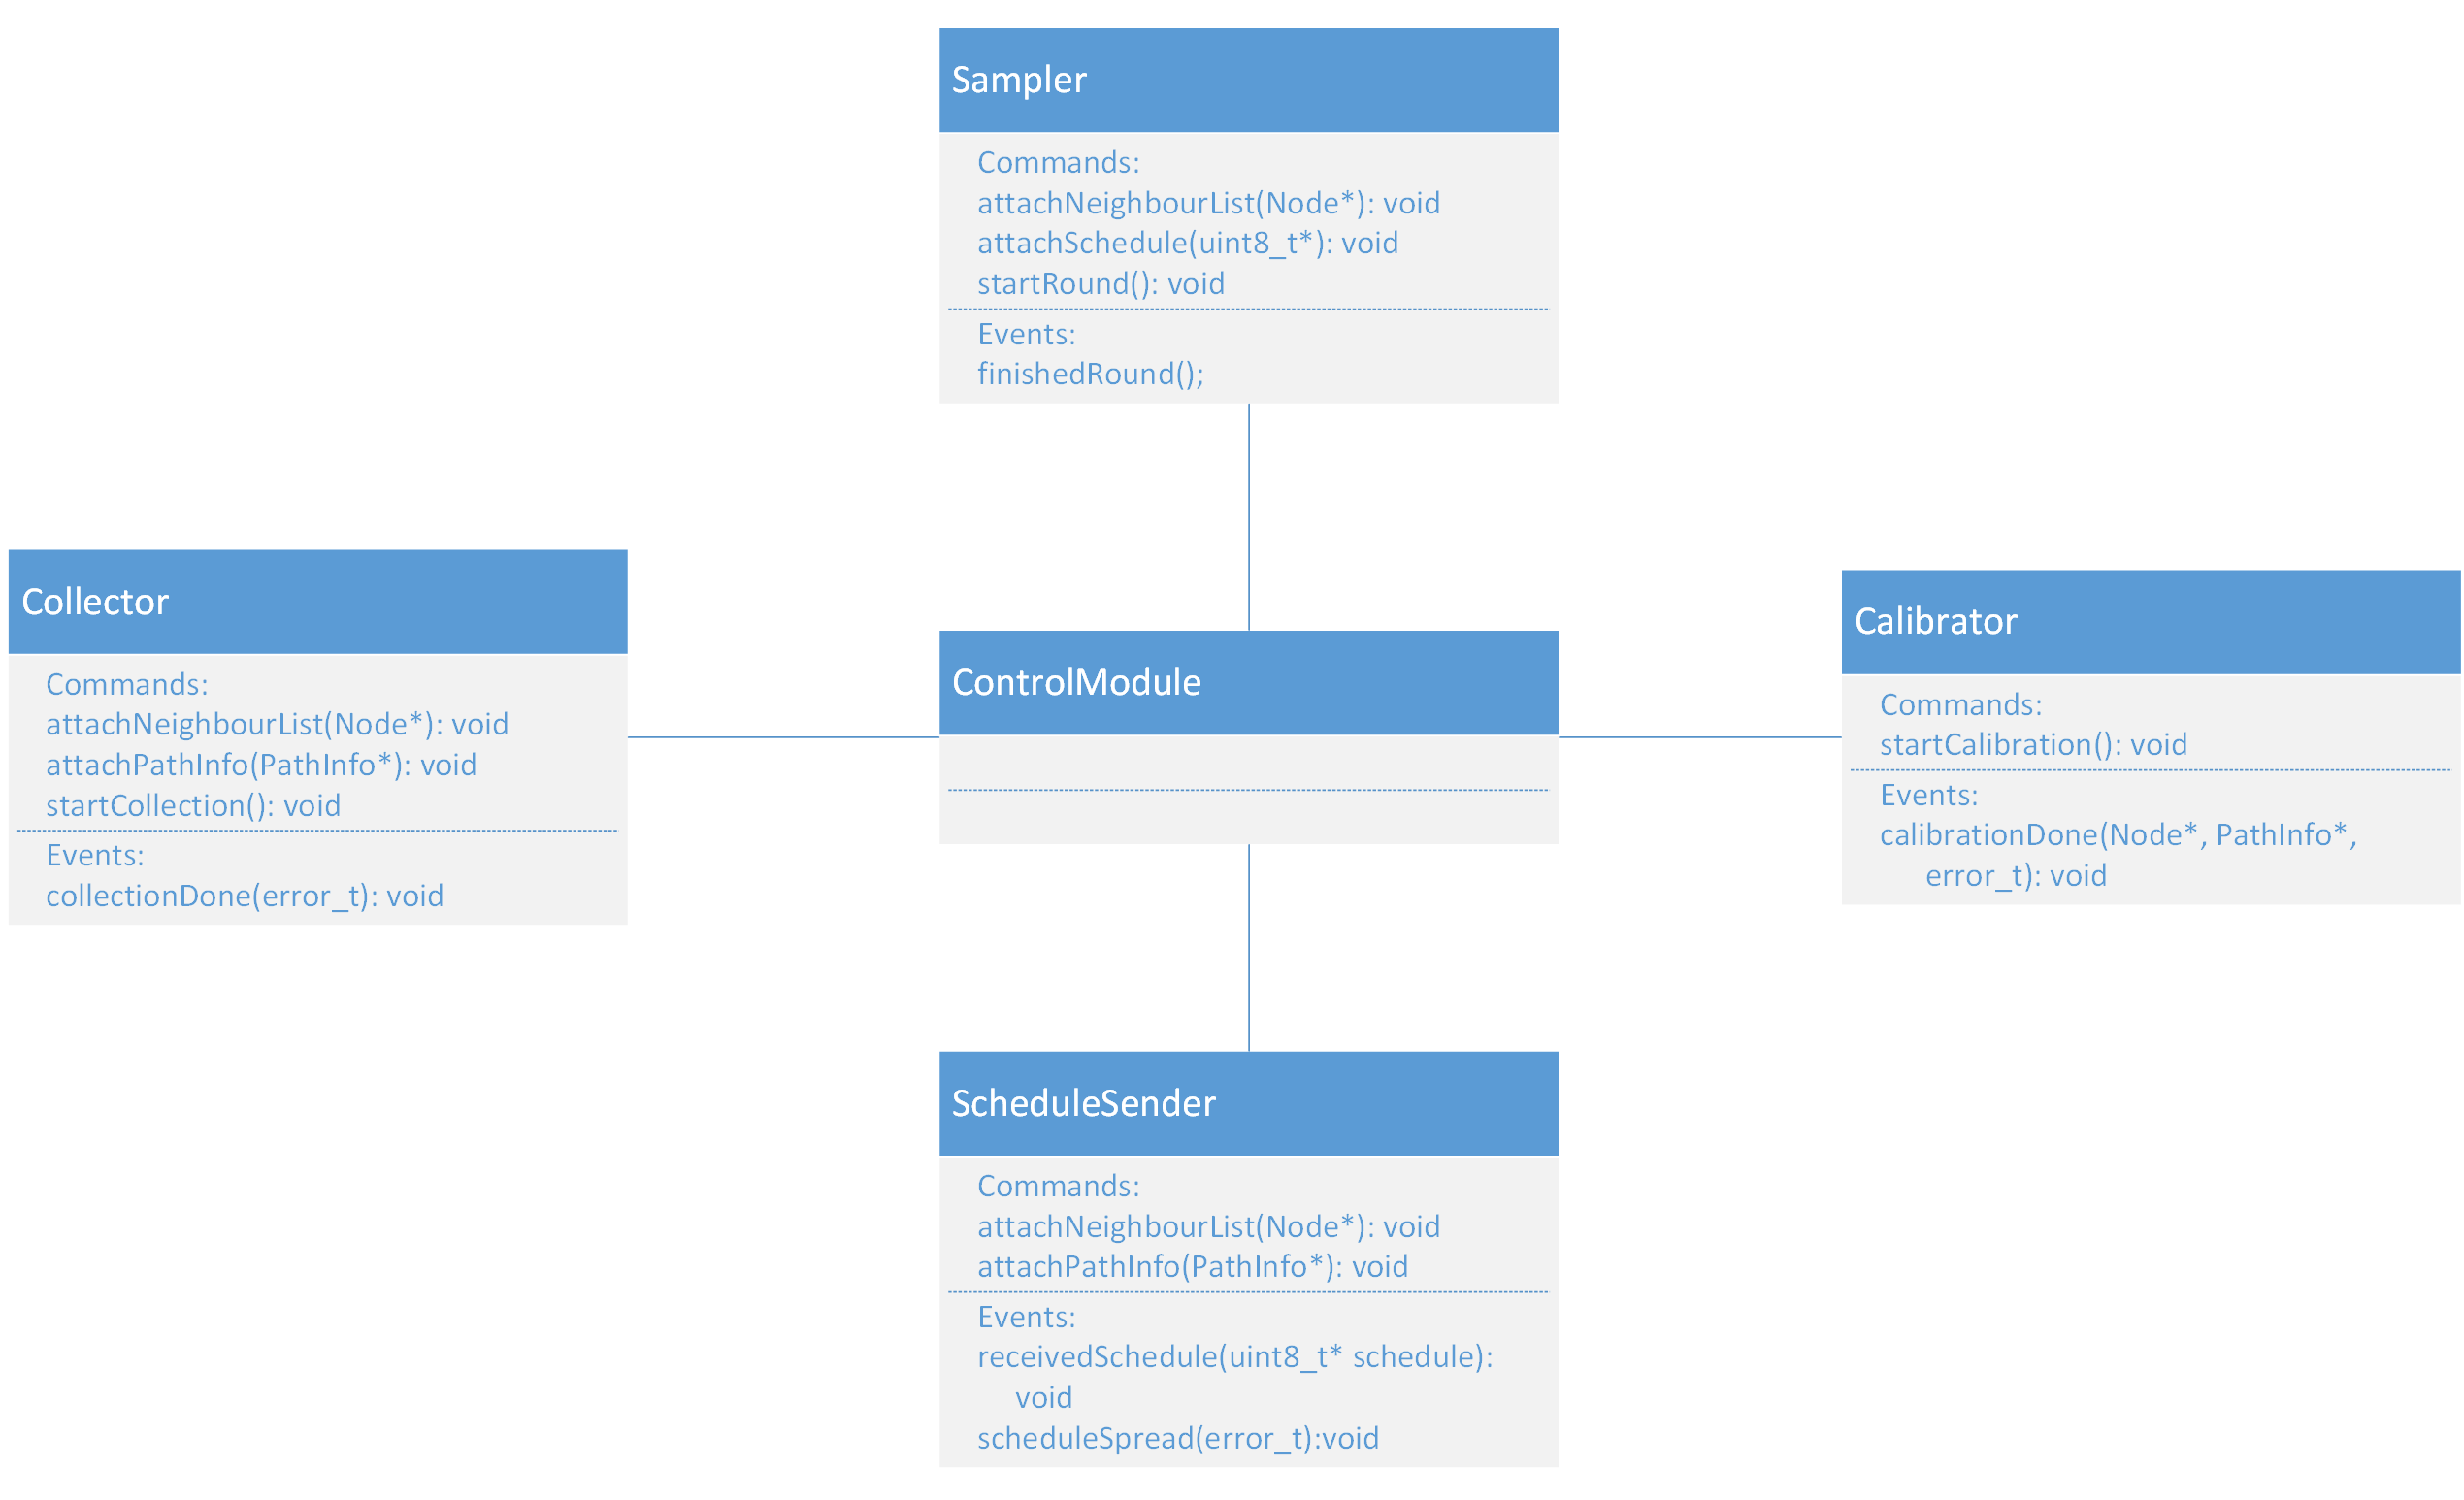
\includegraphics[scale=0.6]{content/images/Motes/GeneralStructure}
   	\caption{The interfaces each module provides. The ControllModule does only use all the other interfaces and does not provide one itself}
    \label{fig:moteStructure}
\end{figure}
\todo{Grafic: attach statt attache und spread statt spreaded, neighbourlist}
The application running on the motes has multiple tasks. It needs to be able to calibrate the network, collect data from the network, spread the schedule inside the network and sample the RSSI. Therefore it can be split into multiple modules with fitting interfaces that each handle exactly one task. The suggested structure of the application is shown in Figure \ref{fig:moteStructure}. The ControllModule connects all the other modules and makes sure the informations the other modules provide get delivered correctly to the modules needing the informations.     
The Calibrator is responsible for the calibration of the network. It needs a command to start the calibration and an event that triggers when the calibration is done and provides the gathered informations. Collecting the data from the network and sending them to the pc is covered by the Collector module. This module needs to know the neighbours and the information about the nodes parent and children. Therefore the interface of the module provides two commands to attach this information to the module. Moreover it needs a event that triggers when the collection is done. To spread the schedule inside the network there is the ScheduleSender module. It also needs the information about the neighbours and the parent and children of the node and has the suitable commands for this. It does not necessary need a command to start the spreading since it can directly react when the node receives a schedule message from the base station. Lastly the module has two events. One that triggers when a node received the schedule and one that triggers when the schedule is spread. The event triggering when the schedule was received provides the received schedule. The schedule spread event will only be triggered at the sink since it is the only node able to detect if the schedule is spread. The last module is the Sampler. It needs the neighbour list and the schedule and has the fitting commands. Moreover it has a command to start one round of the schedule and an event that triggers when this round is finished.  
\section{Base Station}
\subsection{Receiving and Sending messages}
To receive and send messages from the sink it is possible to use the 
\subsection{Storing the information}
\subsection{Creating the Schedule}
\section{Calibration}
\section{Collection}
\section{Creating the Schedule}
\section{Spreading the Schedule}
\section{Sampling}